\documentclass[12pt]{article}%

\usepackage{fancyhdr}
\pagestyle{fancy}
\fancyhf{}
\fancyhead[R]{\thepage}

\usepackage{cmap}				
\usepackage{mathtext} 
\usepackage{listings}

\usepackage{biblatex}
\addbibresource{lib.bib}

\usepackage{euscript}
\usepackage{mathrsfs}

\usepackage[T2A]{fontenc}
\usepackage[utf8]{inputenc}
\usepackage[english,russian]{babel}
\usepackage{amsmath,amsfonts,amssymb,amsthm,mathtools}

\setlength\fboxsep{3pt}
\setlength\fboxrule{1pt}

\usepackage{graphicx}
\usepackage{hyperref}
\usepackage[usenames,dvipsnames,svgnames,table,rgb]{xcolor}
\usepackage{wrapfig}
\hypersetup{				
    unicode=true,           
    pdftitle={Заголовок},   
    pdfsubject={Тема},      
    pdfkeywords={keyword1} {key2} {key3},
    colorlinks=true,
    linkcolor=black,
    citecolor=black,
    filecolor=magenta,
    urlcolor=cyan
}

% Работа с Python
\usepackage{minted}
\definecolor{LightGray}{gray}{0.98}

% Работа с enumerate
\usepackage{enumitem}

\newcommand*{\Title}{\begingroup
\centering 

\large {Федеральное автономное образовательное учреждение высшего образования}
\vspace*{\baselineskip}

\large {«Национальный исследовательский университет «Высшая школа экономики»»}
\vspace*{\baselineskip}

\vspace*{\baselineskip}
\large{\textbf{Отчет по лабораторной работе 1}}

\vspace{0.1cm}
\large{Теория погрешностей и машинная арифметика}

\vspace{0.2cm}
\large{Вариант 10: задачи 1.1.10, 1.3.3, 1.6, 1.7, 1.9.4}

\vspace{1.5cm} 

\begin{flushright}
  \textbf{\normalsize Выполнил:}
  
  \vspace{0.3cm} 
  {\normalsize Студент группы БПМ-211}
  
  {\normalsize Ляхов Артём Андреевич}

\end{flushright}


\vspace{0.2cm}  
\begin{flushright}
  \textbf{\normalsize Преподаватель:} 

  \vspace{0.2cm}

 {\normalsize Брандышев Петр Евгеньевич}
 
\end{flushright}

\vfill
\date{}{Январь 2024 г.}



\endgroup\clearpage}

\begin{document}
\Title
\tableofcontents
\newpage
\section{Задача 1.1.10. Вычисление частичных сумм ряда}
\subsection{Формулировка задачи}
Дан ряд $\sum\limits_{n=0}^{\infty} a_n$, необходимо аналитически найти его сумму, вычислить для $N = 10,\ 10^2,\ 10^3,\ 10^4,\ 10^5$  частичные суммы $S_N = \sum\limits_{n=0}^{N} a_n$, после чего найти и сравнить абсолютные погрешности а также количество верных цифр.

Члены ряда при этом заданы соотношением (задача 1.1.10):
\begin{equation*}
    a_n = \frac{84}{13(n^2 + 14n + 48)}
\end{equation*}

\subsection{Теоретический материал}
Пусть $a$ - точное значение, $a^{*}$ - приближённое значение некоторой величины. \textit{Абсолютной погрешностью} приближённого значения $a^{*}$ называется величина $\Delta(a^{*}) = |a - a^{*}|$. Поскольку точное значение $a$, как правило, неизвестно, чаще получают оценку вида $|a - a^{*}| \leqslant \overline{\Delta}(a^{*})$, где $\overline{\Delta}(a^{*})$ называют \textit{верхней границей абсолютной погрешности}.

Значащую цифру числа $a$ называют \textit{верной}, если абсолютная погрешность числа не превосходит единицы разряда, соответствующего этой цифре.

Абсолютную погрешность $S_N$ можно определить с помощью функции $d(N) = |S_N - S|$, где $S$ - искомая сумма ряда. 

\subsection{Аналитический вывод суммы ряда}
Пусть $S$-искомая сумма ряда, то есть
\begin{equation*}
S = \lim\limits_{N \rightarrow \infty} S_N
\end{equation*}
Разложим дробь $a_n$ на простейшие:
\begin{equation*}
a_n = \frac{84}{13(n + 6)(n + 8)} = \frac{84}{13}\left(\frac{A}{n + 6} + \frac{B}{n + 8} \right)
\end{equation*}

Методом вычёркивания получаем, что $A = \frac{1}{2}$, $B = -\frac{1}{2}$, а значит:
\begin{equation*}
    a_n = \frac{42}{13}\left(\frac{1}{n+6} - \frac{1}{n+8} \right)
\end{equation*}

Таким образом, мы можем выразить частичную сумму ряда как
\begin{equation*}
    S_N = \frac{42}{13}\sum\limits_{n=0}^{N}
    \left(\frac{1}{n + 6} - \frac{1}{n + 8} \right) = 
    \frac{42}{13}\left(\frac{1}{6} + \frac{1}{7} 
    - \frac{1}{N + 7} - \frac{1}{N + 8} \right)
\end{equation*}

Следовательно, итоговая сумма ряда будет равна:
\begin{equation}
    S = \lim\limits_{N \rightarrow \infty} S_N = 
    \frac{42}{13}\left(\frac{1}{6} + \frac{1}{7}\right) = \frac{42}{13}\cdot \frac{13}{42} = 1
\end{equation}


\subsection{Код программы}
Код программы для  эксперимента можно найти в ноутбуке, прикриплённом вместе с отчётом.


\subsection{Результаты вычислительного эксперимента}
В таблице \ref{table:series_res} представлены результаты вычислительного эксперимента, проведённого с использованием языка программирования Python.

\begin{table}[!h]
\begin{center}
    \begin{tabular}{|c|c|c|c|}
    \hline  $N$  &  $S_N$  & Абсолютная погрешность & Количество верных цифр  \\
    \hline  $10$  & 0.630468 & $3.696 \cdot 10^{-1}$   & 0  \\            
    \hline  $10^2$ & 0.939891 & $6.011 \cdot 10^{-2}$  & 1  \\     
    \hline  $10^3$ & 0.993587 & $6.413 \cdot 10^{-3}$  & 2  \\
    \hline  $10^4$ & 0.999354 & $6.457 \cdot 10^{-4}$  & 3  \\
    \hline  $10^5$ & 0.999935 & $6.461 \cdot 10^{-5}$   & 4  \\
    \hline  
    \end{tabular}
    \caption{Результаты эксперимента.}\label{table:series_res}
\end{center}
\end{table}

\textbf{Вывод:} Как видно из результатов эксперимента, увеличение числа суммируемых членов ряда в 10 раз по сравнению с предыдущем случаем увеличивает количество верных цифр на одну. 


\subsection{Гистограммы}

\begin{figure}[!h]
    \centering
    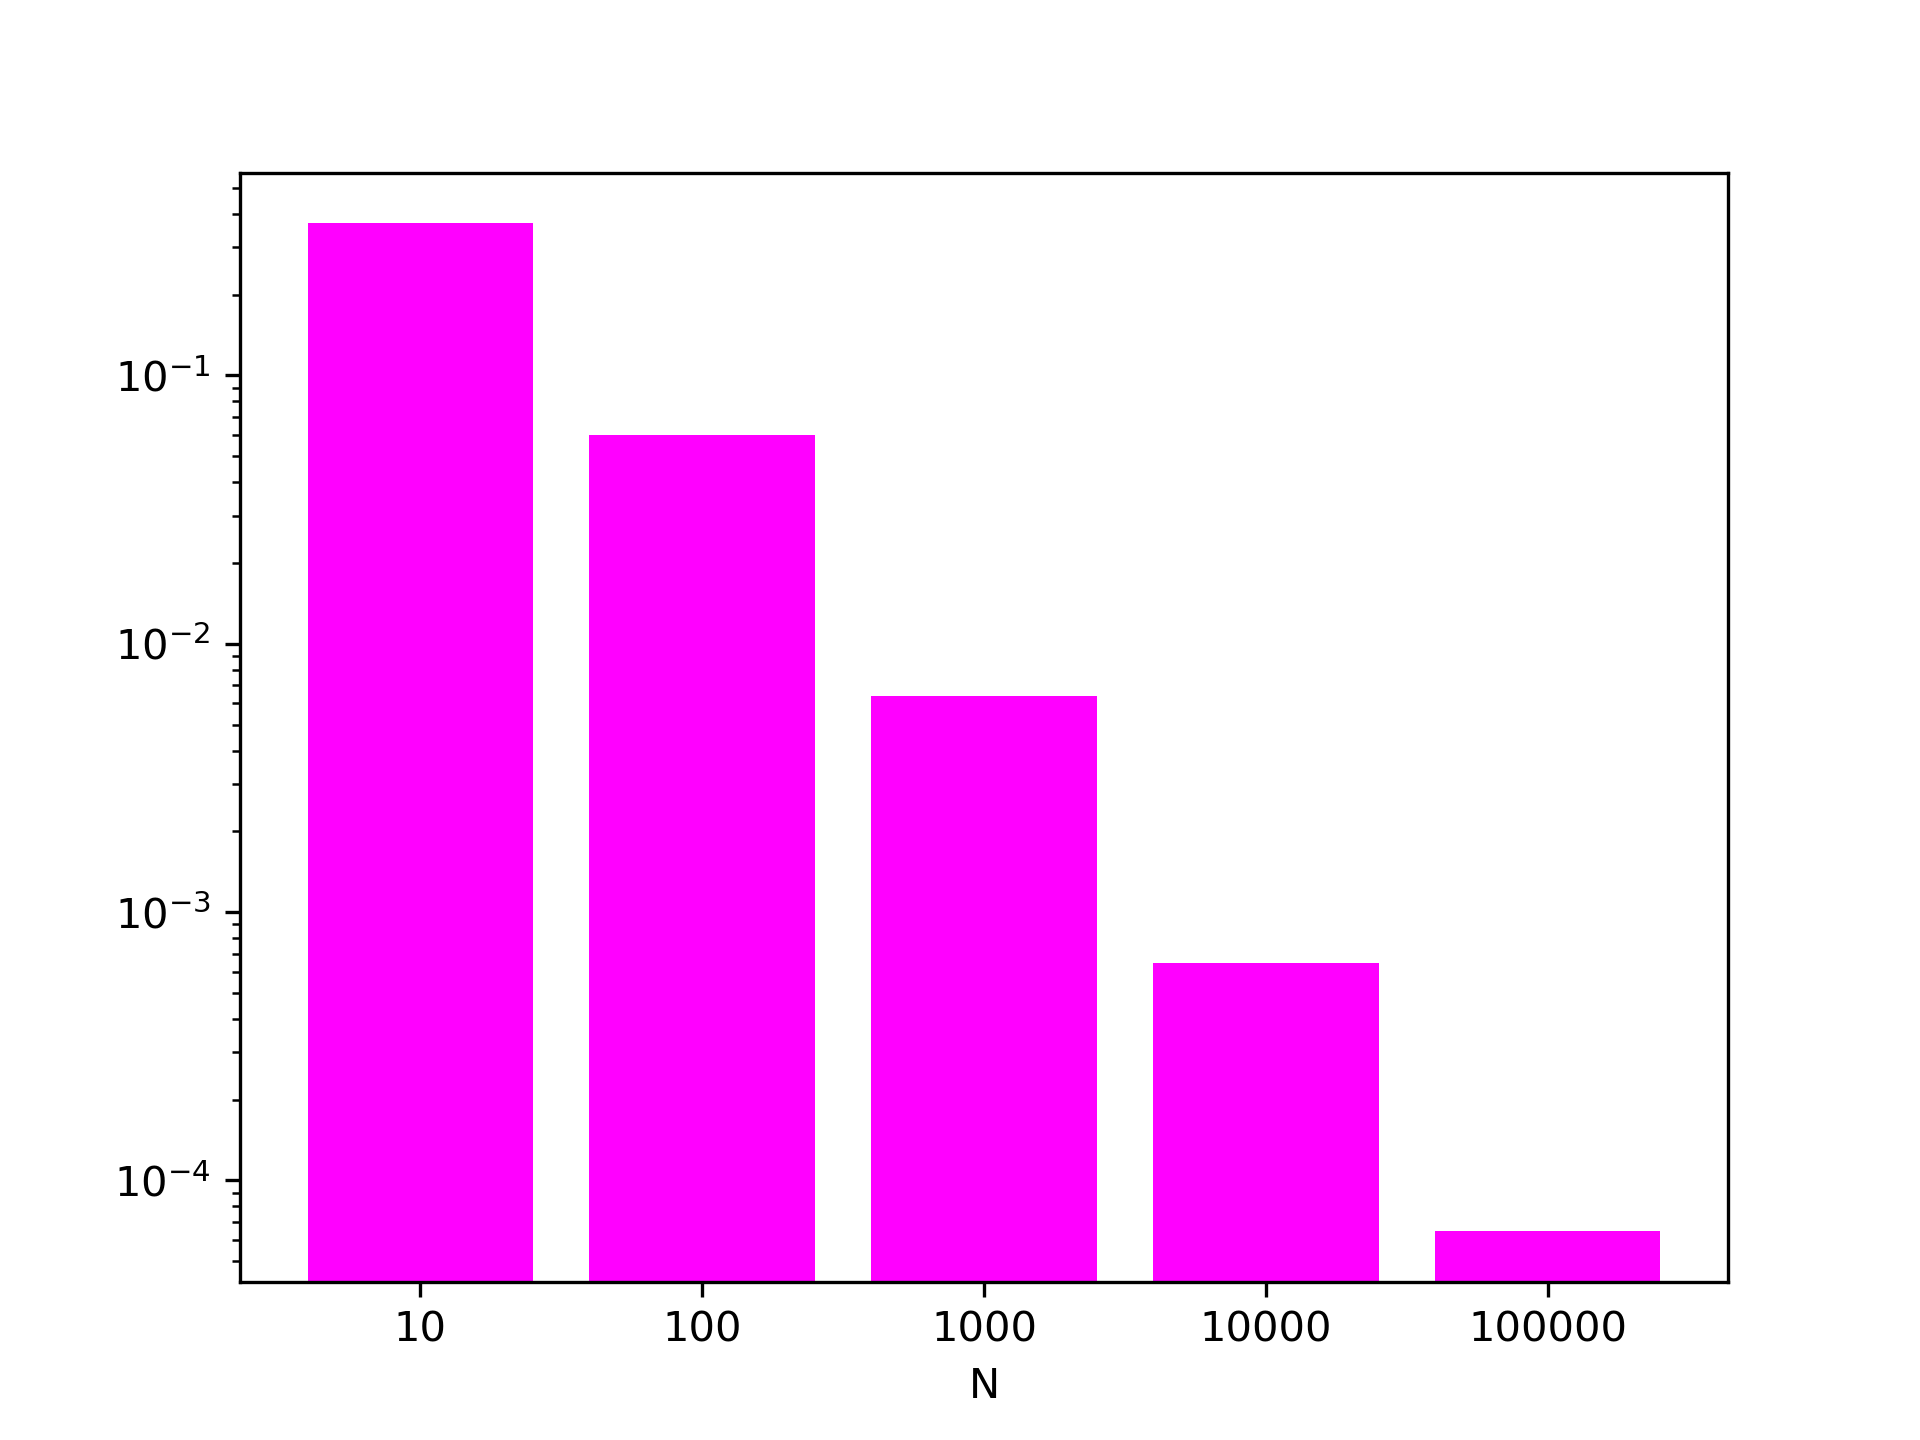
\includegraphics[height=6.5cm]{series_abs_error.png}
    \caption{Гистограмма зависимости абсолютной погрешности $a(S_N)$ от количества суммируемых членов ряда $N$.}
    \label{fig:series_error}
\end{figure}
\newpage

\begin{figure}[!h]
    \centering
    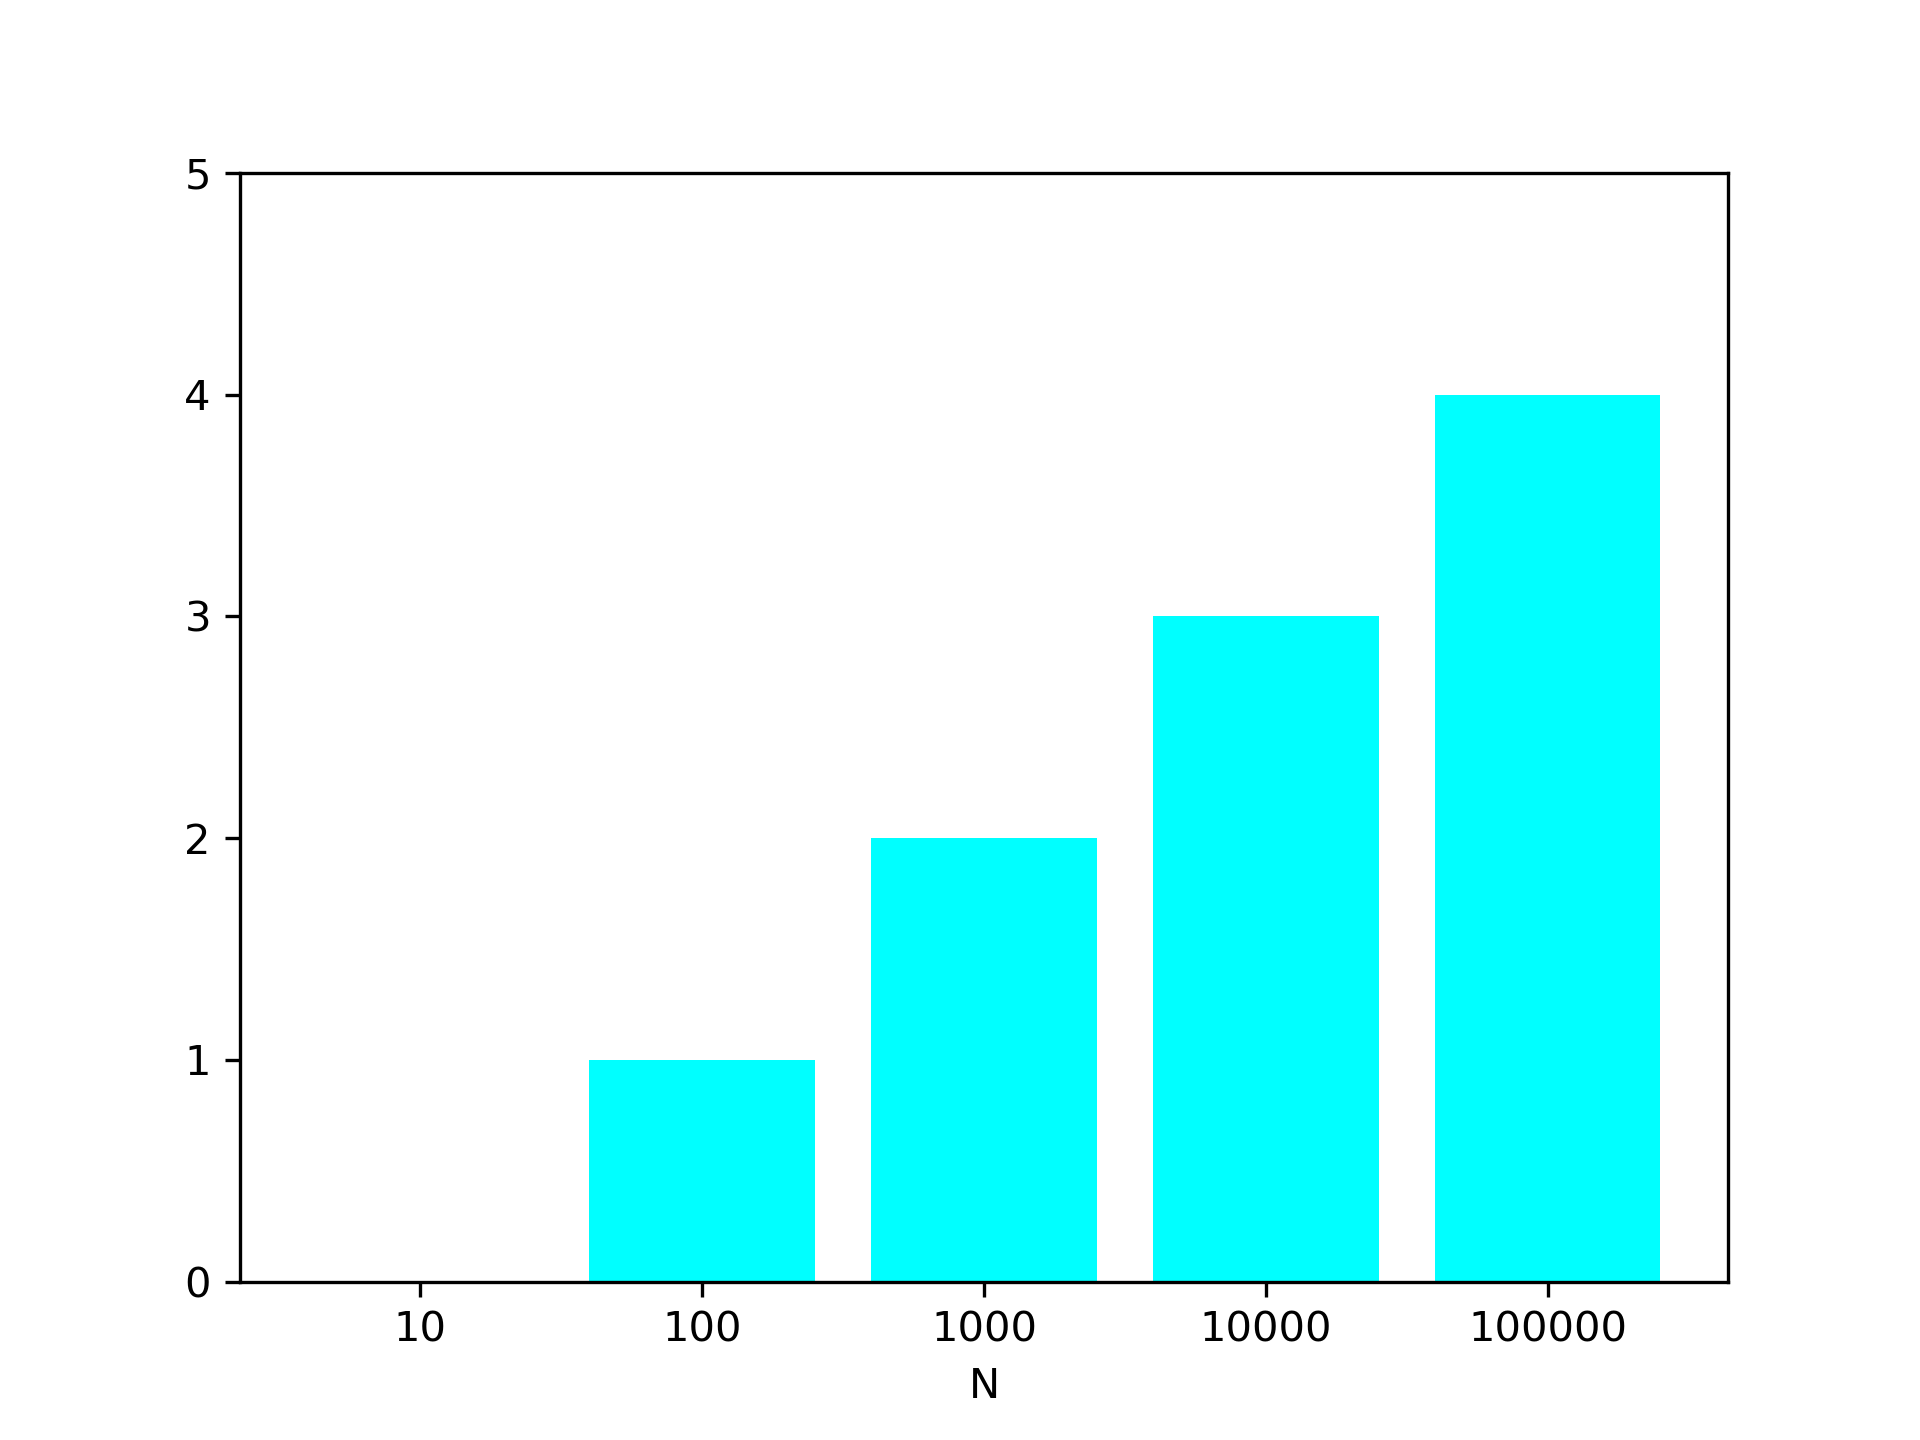
\includegraphics[height=6.5cm]{series_num_digits.png}
    \caption{Гистограмма зависимости количества верных знаков $S_N$ от количества суммируемых членов ряда $N$.}
    \label{fig:series_digits}
\end{figure}
\newpage 


\newpage
\section{Задача 1.3.3. Вычисление обратной матрицы}
\subsection{Формулировка задачи}
Для заданной матрицы $A$ найти (если это возможно) обратную. Затем в элемент $a_{11}$ внести погрешность в 10\% и снова найти обратную. Объяснить полученные результаты. 
\[
A = 
\begin{pmatrix}
    a_{11} & a_{12} & a_{13} \\
    a_{21} & a_{22} & a_{23} \\
    a_{31} & a_{32} & a_{33}
\end{pmatrix} =
\begin{pmatrix}
    3 & 5 & 3 \\
    9 & 15 & 9 \\
    6 & 7 & 2
\end{pmatrix}
\]


\subsection{Результаты вычислений}
Рассмотрим исходную матрицы $A$. Её определитель $\det A = 0$, следовательно, у матрицы $A$ нет обратной.

Для случая $a_{11} = 3.3$ у $A$ сущестует обратная и она равняется:
\begin{equation*}
    \begin{pmatrix}
        3.3 & 5 & 3  \\
        9 & 15 & 9   \\
        6 & 7  & 2
    \end{pmatrix}^{-1} = 
    \begin{pmatrix}
        3.3333 & -1.1111 & 1.1719\cdot10^{-16} \\
        -3.6364 &  1.1515 & 0.27273             \\
        2.7273 & -0.6969 & -0.4545
    \end{pmatrix}
\end{equation*}

Если же $a_{11} = 2.7$ у матрицы $A$ также существует обратная:
\begin{equation*}
   \begin{pmatrix}
        2.7 & 5 & 3  \\
        9 & 15 & 9   \\
        6 & 7  & 2
    \end{pmatrix}^{-1} =
    \begin{pmatrix}
        -3.3333 & 1.1111  & 1.1719\cdot10^{-16} \\
        3.6364  & -1.2727 & 0.27273             \\
        -2.7273 & 1.1212  & -0.4545
    \end{pmatrix}
\end{equation*}

\textbf{Вывод:} Как мы видим, у обраных матриц совпадают третьи столбцы, существенно отличаются вторые столбцы, а первые столбцы имеют противоположные знаки. Таким образом, добавление погрешности в один элемент матрицы может не только повлиять на факт существования обратной матрицы, но и сильно изменить её.

\subsection{Объяснение результата}
Введём дополнительное обозначение
\[
f(\delta) = \begin{pmatrix}
    3 (1 + \delta) & 5 & 3 \\
    9              & 15 & 9 \\
    6              & 7  & 2
\end{pmatrix}
\]
тогда $\det f(\delta) = -99 \delta$. 

Если мы составим матрицу алгебраических дополнений элементов матрицы $A$, то мы увидим, что в ней есть элементы, которые не зависят от $\delta$. Таким образом, в матрице $A^{-1}$ (при условии её существования) есть элементы обратно пропорциональные $\delta$. Это объясняет тот факт, что для $\delta = 0.1$ и $\delta = -0.1$ обратные матрицы очень сильно отличаются друг от друга.

\newpage
\section{Задача 1.6. Машинная точность для Python}
\subsection{Формулировка задачи}
Требуется для Python найти значение машинного нуля, машинной бесконечности, машинного эпсилон.

\subsection{Результаты вычислительно эксперимента}
\begin{table}[!h]
    \centering
    \begin{tabular}{|c|c|}
         \hline Величина & Приближённое значение \\
         \hline Машинный нуль $X_0$ & $5 \cdot 10^{-324}$ \\
         \hline Машинная бесконечность $X_{\infty}$ & $8.99 \cdot 10^{307}$ \\
         \hline Машинное эпсилон $\varepsilon_M$ & $2.22 \cdot 10^{-16}$ \\
         \hline
    \end{tabular}
    \caption{Результаты вычислительного эксперимента, проведённого с использованием Python.}
    \label{tab:my_label}
\end{table}


\subsection{Код программы}
Ниже представлены коды программы для выполнения вычислительного эксперимента.

\begin{minted}[
frame=single,
framesep=10pt,
framerule=0.1pt,
bgcolor=LightGray
]{python}
a = 1
b = a
while a > 0:
    b = a
    a /= 2

print(f"Machine zero in Python is {b}")
\end{minted}
\newpage
\begin{minted}[
frame=single,
framesep=10pt,
framerule=0.1pt,
bgcolor=LightGray
]{python}
a = 1.0
b = a
while a != float('inf'):
    b = a
    a *= 2

print(f"Machine infinity in Python is {b}")
\end{minted}

\begin{minted}[
frame=single,
framesep=10pt,
framerule=0.1pt,
bgcolor=LightGray
]{python}
a = 1.0
eps = a
while a + 1 > 1:
    eps = a
    a /= 2

print(f"Machine epsilon in Python is {eps}")
\end{minted}

\newpage
\section{Задача 1.7. Параметры ЭВМ в разных режимах точности}
\subsection{Формулировка задачи}
Вычислить значения машинного нуля, машинной бесконечности, машинного эпсилон в режимах одинарной, двойной и расширенной точности на двух алгоритмических языках. Сравнить результы.

В рамках решения будем искать параметры ЭВМ на языках Python (пакет numpy) и C++.


\subsection{Результаты вычислительного эксперимента}

\begin{table}[h]
\centering
\begin{tabular}{|c|c|c|}
\hline Величина             & Python         & C++  \\
\hline Машинный нуль 
    & $1.402 \cdot 10^{-45}$ & $1.401 \cdot 10^{-45}$ \\
\hline Машинная бесконечность 
    & $1.701 \cdot 10^{38}$  & $3.402 \cdot 10^{38}$ \\
\hline Машинное эпсилон 
    & $1.192 \cdot 10^{-7}$  & $1.19 \cdot 10^{-7}$ \\
\hline
    \end{tabular}
    \caption{Результаты эксперимента для режима \textbf{одинарной точности}: тип \textit{np.single} для языка Python и \textit{float} для языка C++.}
\end{table}

\begin{table}[h]
\centering
\begin{tabular}{|c|c|c|}
\hline Величина  &  Python  &  C++ \\
\hline Машинный нуль        
    & $5 \cdot 10^{-324}$ & $4.94 \cdot 10^{-324}$ \\
\hline Машинная бесконечность
    & $8.99 \cdot 10^{307}$ & $1.78 \cdot 10^{308}$ \\
\hline Машинное эпсилон
    & $2.22 \cdot 10^{-16}$ & $2.22 \cdot 10^{-16}$ \\
\hline
    \end{tabular}
    \caption{Результаты эксперимента для режима \textbf{двойной точности}: тип \textit{np.double} для языка Python и \textit{double} для языка C++.}
\end{table}

\begin{table}[h]
    \centering
\begin{tabular}{|c|c|c|}
\hline Величина &  Python  &  C++ \\
\hline Машинный нуль
    & $5 \cdot 10^{-324}$ & $3.64 \cdot 10^{-4951}$ \\
\hline Машинная бесконечность
    & $8.988 \cdot 10^{307}$ & $1.19 \cdot 10^{4932}$ \\
\hline Машинное эпсилон
    & $2.22 \cdot 10^{-16}$ & $1.08 \cdot 10^{-19}$ \\
\hline
\end{tabular}

\caption{Результаты эксперимента для режима \textbf{расширенной точности}:
тип \textit{np.longdouble} для языка Python и \textit{long double} для языка C++}.
\end{table}

\newpage
\textbf{Вывод:} Как мы видим, в режимах одинарной и двойной точности приближённые значения параметров совпадают. В то же время для режима расширенной точности наблюдается огромное расхождение. Скорее всего, это связано с тем, что пакет numpy на текущий момент полноценно не поддерживает режим расширенной точности.

\subsection{Код программы}
Код для проведения эксперимента на языке Python можно найти в файле \textbf{laboratory\_work1.ipynb}, на языке C++ в файле \textbf{lr1\_exp.cpp}. Оба файла прикреплены вместе с отчётом.

\newpage
\section{Задача 1.9.4 Существование обратной матрицы}
\subsection{Формулировка задачи}
Для матрицы $A$ решить вопрос существования обратной матрицы в следующих случаях:
\begin{enumerate}
    \item[1)] элементы матрицы заданы точно;
    \item[2)] элементы матрицы заданы приближённо с относительной погрешностью а)$\delta = \alpha \%$  б)$\delta = \beta \%$.
\end{enumerate}
Найти относительную погрешность результата.
\begin{equation*}
    A = \begin{pmatrix}
        9 & 5 & 6 \\
        13.5 & 9.5 & 11 \\
        8    & 4   & 5
    \end{pmatrix}
\end{equation*}
\begin{equation*}
    \alpha = 0.1\ \ \ \ \ \beta = 0.5
\end{equation*}

\subsection{Теоретический материал}
У квадратной матрицы существует обратная тогда и только тогда, когда её определитель не равен нулю. Таким образом, наша задача полностью сводится к нахождению определителя и сравнению его с нулём.

В случае, когда все элементы матрицы заданы точно, можно найти точное значение определителя и дать правильный ответ на вопрос задачи.

В случае, когда элементы матрицы (а, следовательно, и определителя) заданы приближённо с относительной точностью $\delta$ дело обстоит сложнее. Если обозначить за $a_{ij}$ элементы матрицы $A$, то каждый элементы $a_{ij}$ может принимать любое значение из отрезка 
$[a_{ij}(1 - \delta),\ a_{ij}(1 + \delta )]$,
если $a_{ij} \geqslant 0$ и из отрезка
$[a_{ij}(1 + \delta),\ a_{ij}(1 - \delta )]$,
если $a_{ij} < 0$. Множество всех возможных элементов матрицы значений матрицы $A$ представляет компакт в 9-мерном пространстве. Сам определитель является дифференцируемой функцией девяти переменных - элементов матрицы $a_{ij}$. По теореме Вейерштрасса эта функция достигает на указанном множестве своего максимального и минимального значений - $M$ и $m$, соответственно. Если отрезок $[m, M]$ не содержит точку 0, то при любых допустимых значениях $a_{ij}$ определитель не равен нулю, и следовательно, у матрицы $A$ существует обратная. Если $0 \in [m, M]$, то рассуждения выше неправомерные и будет иметь место неопределённость.

Нахождению $m$ и $M$ помогает одно очень полезное утверждение. Как функция от элементов матрицы определитель всегда достигает максимума и минимума на границе области, и более того, координаты этих точек имеют вид $a_{ij}(1 \pm \delta)$. Таким образом, для нахождения $m, M$ нужно посчитать определитель в $2^9 = 512$ точка и выбрать из значений максимальное и минимальное значения.

Относительная погрешность может быть оценена сверху как 
$\frac{\overline{\Delta}(a^{*})}{|a^{*}|}$, где $\overline{\Delta}(a^{*}) = \frac{1}{2}\left(M - m\right)$, $a^{*} = \frac{M + m}{2}$ - середина отрезка $[m, M]$.

\subsection{Результаты вычислительного эксперимента}
\subsubsection{Случай точных значений}
Если значения матрицы $A$ заданы точно, то $\det(A) = 2 \ne 0$. Следовательно, у матрицы $A$ существует обратная $A^{-1}$. 

\subsubsection{Случай приближённых значений}
\begin{table}[h]
\centering
\begin{tabular}{|c|c|c|c|}    
\hline $\delta$           & $m$     & $M$    & Относительная погрешность \\
\hline $\alpha\% = 0.001$ & 1.4695  & 2.5295 & 0.265 \\
\hline $\beta\% = 0.005$  & -0.6632 & 4.6367 & 1.334 \\
\hline
\end{tabular}
\caption{Результаты вычисления $m$ и $M$ для различных значений $\delta$. }
\end{table}

\textbf{Вывод:} Для случая $\delta = \alpha \%$ мы можем утверждать, что обратная матрица существует, в то время как в случае $\delta = \beta \%$ возникает неопределённость и мы не можем сделать о вывод о том, существует обратная матрица или нет.

\subsection{Код программы}
Код программы находится в файле \textbf{laboratory\_work1.ipynb}, прикреплённом вместе отчётом.


\end{document}